%%%%%%%%%%%%%%%%%%%%%%%%%%%%%%%%%%%%%%%%%
% Programming/Coding Assignment
% LaTeX Template
%
% This template has been downloaded from:
% http://www.latextemplates.com
%
% Original author:
% Ted Pavlic (http://www.tedpavlic.com)
%
% Note:
% The \lipsum[#] commands throughout this template generate dummy text
% to fill the template out. These commands should all be removed when 
% writing assignment content.
%
% This template uses a Perl script as an example snippet of code, most other
% languages are also usable. Configure them in the "CODE INCLUSION 
% CONFIGURATION" section.
%
%%%%%%%%%%%%%%%%%%%%%%%%%%%%%%%%%%%%%%%%%

%----------------------------------------------------------------------------------------
%	PACKAGES AND OTHER DOCUMENT CONFIGURATIONS
%----------------------------------------------------------------------------------------

\documentclass{article}

\usepackage{fancyhdr} % Required for custom headers
\usepackage{lastpage} % Required to determine the last page for the footer
\usepackage{extramarks} % Required for headers and footers
\usepackage[usenames,dvipsnames]{color} % Required for custom colors
\usepackage{graphicx} % Required to insert images
\usepackage{listings} % Required for insertion of code
\usepackage{courier} % Required for the courier font
\usepackage{lipsum} % Used for inserting dummy 'Lorem ipsum' text into the template
\usepackage{amssymb,amsmath}
\usepackage{xcolor}
\usepackage{float}
\usepackage{enumitem}
\usepackage{subcaption}
\usepackage{dashbox}					% For making dashed boxes around equations
\restylefloat{figure}
\usepackage{microtype}	
% Margins
\topmargin=-0.45in
\evensidemargin=0in
\oddsidemargin=0in
\textwidth=6.5in
\textheight=9.0in
\headsep=0.25in

\linespread{1.1} % Line spacing

% Set up the header and footer
\pagestyle{fancy}
\lhead{} % Top left header
\rhead{} % Top center head
\chead{\hmwkClass: \hmwkTitle} % Top right header
\cfoot{\hmwkAuthorName} % Bottom left footer
\lfoot{\hmwkDueDate} % Bottom center footer
\rfoot{Page\ \thepage\ of\ \protect\pageref{LastPage}} % Bottom right footer
\renewcommand\headrulewidth{0.4pt} % Size of the header rule
\renewcommand\footrulewidth{0.4pt} % Size of the footer rule
\newcommand{\norm}[1]{\left\lVert#1\right\rVert}
\setlength\parindent{0pt} % Removes all indentation from paragraphs
\newcommand{\ihat}{\hat{\textbf{\i}}}
\newcommand{\jhat}{\hat{\textbf{\j}}}

%----------------------------------------------------------------------------------------
%	CODE INCLUSION CONFIGURATION
%----------------------------------------------------------------------------------------

\definecolor{mygreen}{RGB}{28,172,0} % color values Red, Green, Blue
\definecolor{mylilas}{RGB}{170,55,241}
\lstset{language=matlab,frame=single}

\lstset{language=Matlab,%
    %basicstyle=\color{red},
    breaklines=true,%
    morekeywords={matlab2tikz},
    %keywordstyle=\color{blue},%
    morekeywords=[2]{1}, keywordstyle=[2]{\color{black}},
    identifierstyle=\color{black},%
    stringstyle=\color{mylilas},
    commentstyle=\color{mygreen},%
    showstringspaces=false,%without this there will be a symbol in the places where there is a space
    numbers=left,%
    numberstyle={\tiny \color{black}},% size of the numbers
    numbersep=9pt, % this defines how far the numbers are from the text
    emph=[1]{for,end,break,function,if,elseif,else},emphstyle=[1]\color{blue}, %some words to emphasise
    emph=[2]{ds,dds,curvature,avgcurvature,dact,ddact,marker, kvar, avgkvar, marker_var, marker_repara}, emphstyle=[2]\color{violet},    
}
%----------------------------------------------------------------------------------------
%	DOCUMENT STRUCTURE COMMANDS
%	Skip this unless you know what you're doing
%----------------------------------------------------------------------------------------

% Header and footer for when a page split occurs within a problem environment
\newcommand{\enterProblemHeader}[1]{
\nobreak\extramarks{#1}{#1 continued on next page\ldots}\nobreak
\nobreak\extramarks{#1 (continued)}{#1 continued on next page\ldots}\nobreak
}

% Header and footer for when a page split occurs between problem environments
\newcommand{\exitProblemHeader}[1]{
\nobreak\extramarks{#1 (continued)}{#1 continued on next page\ldots}\nobreak
\nobreak\extramarks{#1}{}\nobreak
}

\setcounter{secnumdepth}{0} % Removes default section numbers
\newcounter{homeworkProblemCounter} % Creates a counter to keep track of the number of problems

\newcommand{\homeworkProblemName}{}
\newenvironment{homeworkProblem}[1][Problem \arabic{homeworkProblemCounter}]{ % Makes a new environment called homeworkProblem which takes 1 argument (custom name) but the default is "Problem #"
\stepcounter{homeworkProblemCounter} % Increase counter for number of problems
\renewcommand{\homeworkProblemName}{#1} % Assign \homeworkProblemName the name of the problem
\section{\homeworkProblemName} % Make a section in the document with the custom problem count
\enterProblemHeader{\homeworkProblemName} % Header and footer within the environment
}{
\exitProblemHeader{\homeworkProblemName} % Header and footer after the environment
}

\newcommand{\problemAnswer}[1]{ % Defines the problem answer command with the content as the only argument
\noindent\framebox[\columnwidth][c]{\begin{minipage}{0.98\columnwidth}#1\end{minipage}} % Makes the box around the problem answer and puts the content inside
}

\newcommand{\homeworkSectionName}{}
\newenvironment{homeworkSection}[1]{ % New environment for sections within homework problems, takes 1 argument - the name of the section
\renewcommand{\homeworkSectionName}{#1} % Assign \homeworkSectionName to the name of the section from the environment argument
\subsection{\homeworkSectionName} % Make a subsection with the custom name of the subsection
\enterProblemHeader{\homeworkProblemName\ [\homeworkSectionName]} % Header and footer within the environment
}{
\enterProblemHeader{\homeworkProblemName} % Header and footer after the environment
}

%----------------------------------------------------------------------------------------
%	NAME AND CLASS SECTION
%----------------------------------------------------------------------------------------

\newcommand{\hmwkTitle}{Linear Methods for Supervised Learning} % Assignment title
\newcommand{\hmwkDueDate}{March 6, 2020} % Due date
\newcommand{\hmwkClass}{CSE 574: Introduction to Machine Learning - PA 1} % Course/class

\newcommand{\hmwkAuthorName}{Group \# 4} % Your name

%----------------------------------------------------------------------------------------
%	TITLE PAGE
%----------------------------------------------------------------------------------------

\title{
\vspace{2in}
\textmd{\textbf{\hmwkTitle}}\\
\vspace{0.1in}\large{\textit{\hmwkClass}} \\
\normalsize\vspace{0.1in}\small{\hmwkDueDate}
\vspace{3in}
}

\author{\textbf{\hmwkAuthorName}\\ \\ \textbf{Anjali Bachani} \\  \textbf{Abhishek Mishra} \\  \textbf{Adithya L. Narayanan}}
\date{} % Insert date here if you want it to appear below your name

%----------------------------------------------------------------------------------------
\usepackage[none]{hyphenat}

\begin{document}
\maketitle
\thispagestyle{empty}
%----------------------------------------------------------------------------------------
%	TABLE OF CONTENTS
%----------------------------------------------------------------------------------------

%\setcounter{tocdepth}{1} % Uncomment this line if you don't want subsections listed in the ToC

\newpage
\tableofcontents
\vspace{50px}
\listoffigures	



\newpage
\begin{homeworkProblem}[Problem 1: Linear Regression with Direct Minimization]

In this problem, we implement linear regression with direct minimization, using the closed form equation. Root mean squared error (RMSE) used to assess the predictive accuracy of the model. 

\vspace{2ex}
We compare the model performance across two cases: with an intercept (or bias) term and without an intercept term added to the predictors. 

\vspace{2ex}
RMSE without Intercept on train data -  138.20 \\
RMSE with Intercept on train data -  46.77 \\
RMSE without Intercept on test data -  326.76 \\
RMSE with Intercept on test data -  60.89 

\vspace{2ex}
We observe that the error is higher for training and test data without an intercept as compared to that calculated with intercept. 


\end{homeworkProblem}

\begin{homeworkProblem}[Problem 2: Using Gradient Descent for Linear Regression Learning]

In this problem, Gradient Descent, using \texttt{scipy.optimize.minimize} is employed to minimize the linear regression error function. Similar to Problem 1, RMSE is used to measure the predictive accuracy of this model. 

\vspace{2ex}

\vspace{2ex}
Gradient Descent Linear Regression RMSE on train data - 48.08 \\
Gradient Descent Linear Regression RMSE on test data - 54.80

\vspace{2ex}
Based on the model's predictive accuracy, it can be inferred that Gradient Descent performs better in this scenario.

\end{homeworkProblem}


\begin{homeworkProblem}[Problem 3: Using Gradient Descent for Perceptron Learning]

For the scope of this problem, perceptron learning functions as a two class classification method that relies on linear regression's error function, which is minimized using gradient descent. 

\vspace{2ex}
\vspace{2ex}
Perceptron Accuracy on train data - 84 \% \\
Perceptron Accuracy on test data - 84 \%


\end{homeworkProblem}

\begin{homeworkProblem}[Problem 4: Using Newton's Method for Logistic Regression Learning]

The functions \texttt{logisticObjVal}, \texttt{logisticGradient} and \texttt{logisticHessian} were implemented to compute the logistic loss, gradient vector of logistic loss and the Hessian matrix of logistic loss respectively, for the given data set. These functions were then used to train the logistic regression model by calling the \texttt{scipy.optimize.minimize} method. The function \texttt{evaluateLinearModel} from Problem 3 was used to calculate the accuracy of the training and test data. The accuracies obtained are reported as follows:

\vspace{2ex}
Logistic Regression Accuracy on train data - 84 \%\\
Logistic Regression Accuracy on test data - 86 \%




\end{homeworkProblem}

\begin{homeworkProblem}[Problem 5: Using Stochastic Gradient Descent Method for Training Linear Support Vector Machine ]

Using stochastic gradient descent, a linear Support Vector Machine (SVM) is trained to performed binary classification. The accuracy measures for this implementation were a range, due to the stochastic nature of the algorithm which involves random sampling of obervations to update the weights of predictors. 

SVM Accuracy Range on train data: 65-87 \%\\
SVM Accuracy Range on test data: 81-88 \%\\


\end{homeworkProblem}


\begin{homeworkProblem}[Problem 6: Comparing Linear Classifiers]

Comparing the results obtained from Problems 3, 4 and 5, we can say that logistic regression  and SVM classifier give better accuracies in general, however, the results can be a bit sporadic with SVMs due to the stochastic implementation carried out in this study. Even though SVM classifier may sometimes report test accuracy greater than that of logistic regression,  the logistic regression classifier yields higher average accuracy over training and test data and should therefore be preferred to build more robust models. The entropy in the performance can be attributed to the random sampling carried out as a part of the implementation that may fail to capture the true nature of the data it is being tested on at all times (a limited number of observations may not always capture the trend of the data). 

\begin{figure}[H]
    \centering
    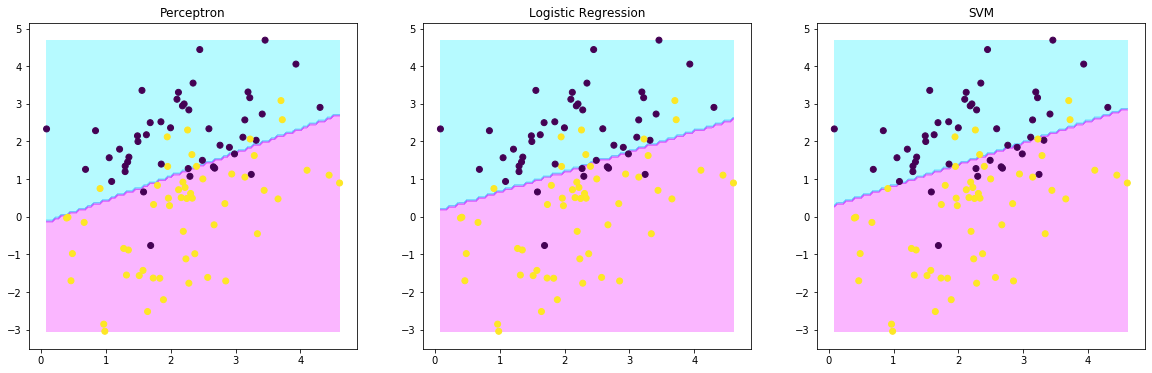
\includegraphics[width=\textwidth]{comparison_plot.png}
    \caption{Decision boundaries learnt by each of the classifiers}
\end{figure}

Observing the decision boundaries in Figure 1, we see that the results from the three classifiers are almost identical. But upon looking more closely, we can see that in this particular case, the SVM classifier has less number of data points on the wrong side of decision boundary. The logistic regression classifier and the perceptron classifier have somewhat equal number of data points on the wrong side of the decision boundary.Iterative runs yield differing decsion boundaries for SVMs, which can again be attributed to the stochastic nature of the process, as described above, wherein each run of training may not necessarily converge with the same decision boundary being learnt. 


\end{homeworkProblem}

%----------------------------------------------------------------------------------------



%----------------------------------------------------------------------------------------
%	APPENDIX
%----------------------------------------------------------------------------------------

%----------------------------------------------------------------------------------------

\end{document}
